\section{Funzionalità disponibili per l'utente}
\label{sec:sezUtente}

Tutte le istruzioni fornite sono riferite all'utilizzo dell'applicativo con il tema chiaro e con il sistema impostato in lingua inglese. Se si ha la necessità di cambiarlo, si veda la sezione 5 (Impostazioni generali).

Una volta entrati nel sistema, l'utente troverà una schermata con in alto: il nome e il simbolo di ChatSql a sinistra e il bottone per le impostazioni e per il login a destra. A sinistra è presente un menù con la voce "Chat" che permette di avere accesso alla finestra della chat per inserire richieste in linguaggio naturale. A destra del menù è presente la scheda principale che rappresenta la chat del sistema e ha un menù in alto. Al centro vengono visualizzate le richieste e le risposte strutturate come una chat di messaggi e in basso è possibile inserire le richieste in linguaggio naturale.

\subsection{Interazione con la chat}

Per interagire con la chat si deve inserire una richiesta nel box di testo in basso. È necessario inserire interrogazioni coerenti con il dizionario dati scelto in modo tale da ricevere la formulazione di un \glossario{prompt} corretto. Le richieste inserite dall'utente nella chat verranno visualizzate a destra con uno sfondo azzurrino mentre le risposte con i prompt generati dal sistema saranno visualizzate a sinistra su sfondo grigio scuro.

\begin{figure}[H]
  \centering
  %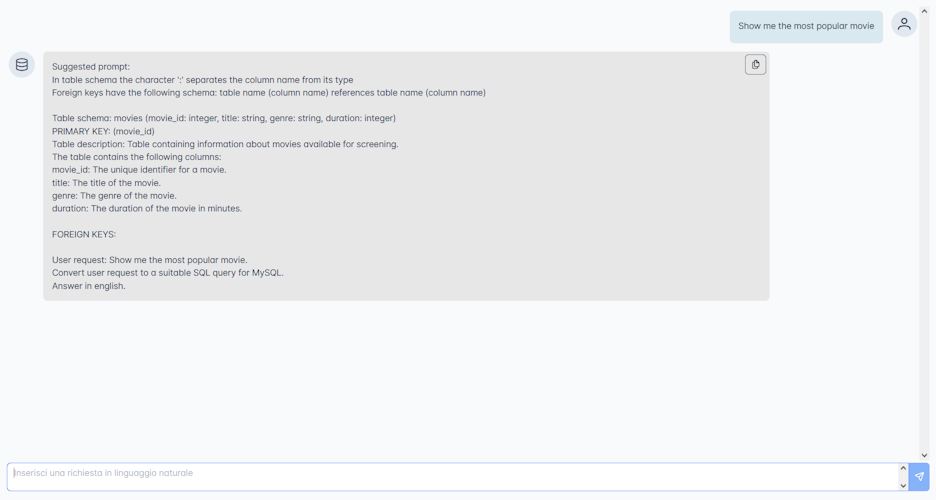
\includegraphics[width=1\textwidth]{assets/chat_example.png}
  \caption{Esempio di interazione nella chat con prompt generato}
\end{figure}

Per inviare una richiesta in linguaggio naturale si deve scrivere nel box di testo, ovvero il rettangolo bianco al centro in basso, con i bordi grigi. Inizialmente alla prima interazione, compare una scritta in grigio chiaro: "Inserisci una richiesta in linguaggio naturale". Terminata la richiesta, è possibile cliccare l'icona di invio, rappresentata con un aeroplanino stilizzato e azzurra in basso a destra affianco al box di testo di inserimento. Questa operazione toglierà il testo scritto dal box di testo per permettere di inserire richieste successive e manterrà la richiesta inviata, riportandola nella chat a destra con lo sfondo azzurro.

\begin{figure}[H]
  \centering
  %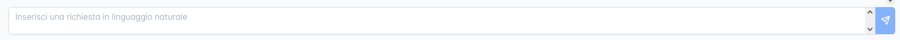
\includegraphics[width=1\textwidth]{assets/text_box_arrow.png}
  \caption{Box di testo e tasto invio}
\end{figure}

È possibile che si verifichino degli errori e il sistema non sia in grado di formulare il \glossario{prompt} data la richiesta. In questo caso è consigliabile controllare il \glossario{dizionario dati} scelto (sezione 6.2.2 - Accesso ad informazioni aggiuntive sul dizionario dati scelto) o se l'interrogazione utilizza i termini corretti e coerenti.

\begin{figure}[H]
  \centering
  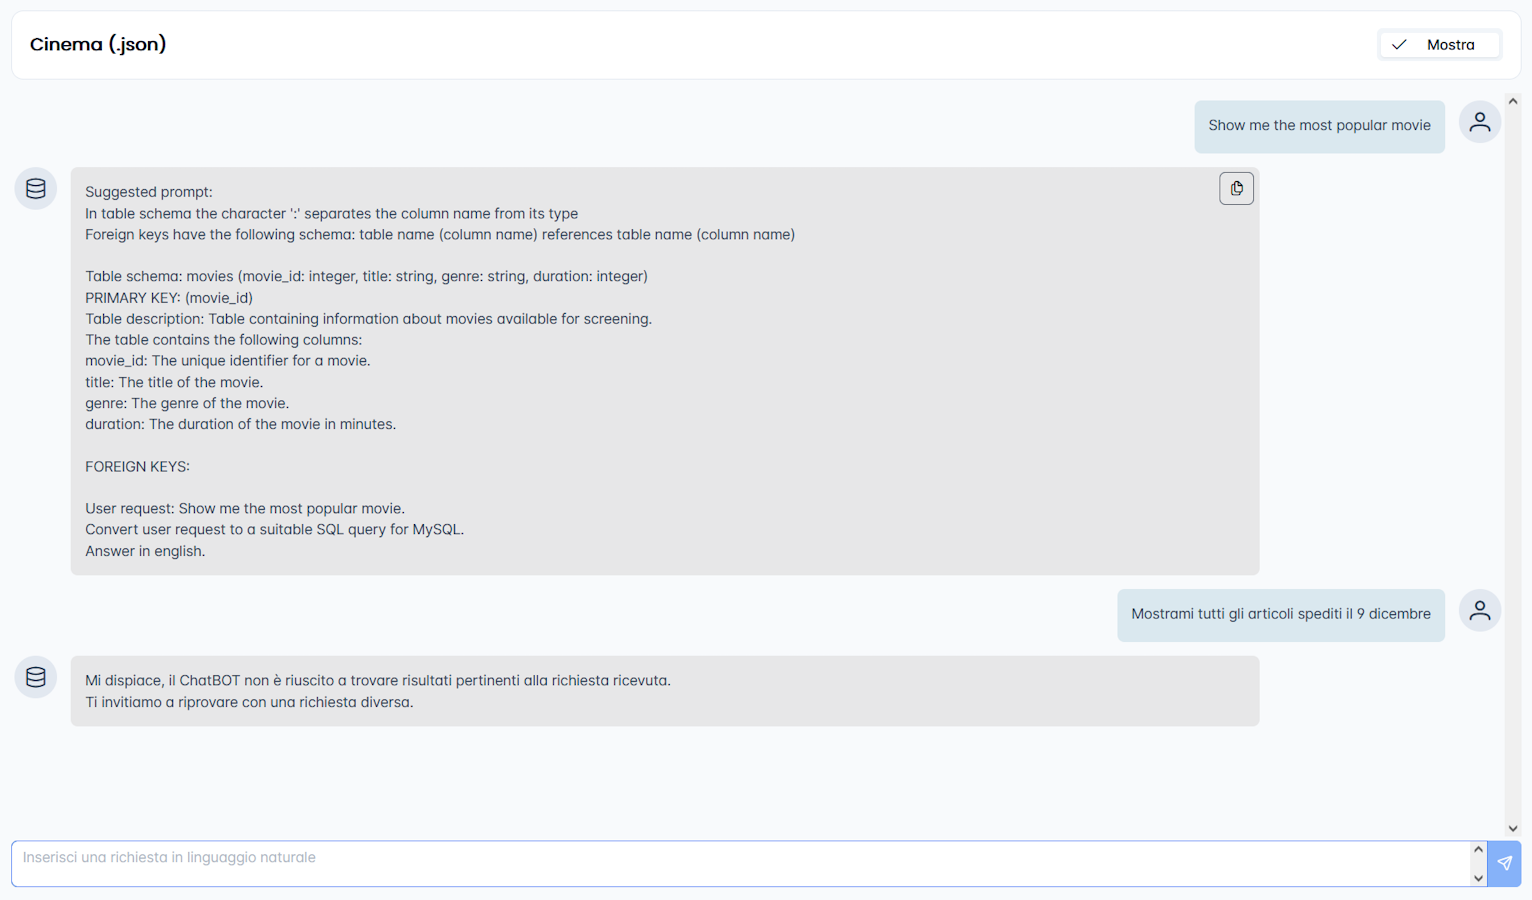
\includegraphics[width=1\textwidth]{assets/es_chat_errore.png}
  \caption{Esempio di errore nel sistema}
\end{figure}

\subsection{Funzionalità impostabili prima e durante l'interazione con la chat}

\begin{enumerate}
  \item Selezione/cambio dizionario dati
  \item Accesso ad informazioni aggiuntive sul dizionario dati scelto
  \item Selezione/cambio DBMS
  \item Selezione/cambio lingua
\end{enumerate}

\subsubsection{Selezione/cambio dizionario dati}

Durante l'interazione con il sistema, è possibile cambiare il \glossario{dizionario dati} su cui basare le richieste inserite in linguaggio naturale. Per fare ciò si deve cliccare il bottone "Mostra" in alto a destra nella chat e una volta aperto il menù il dizionario dati sarà la prima voce a sinistra delle quattro presenti. Il nome che si legge nel box al momento dell'apertura del menù è quello del dizionario dati utilizzato in quel momento. Per cambiare dizionario dati è necessario andare sopra con il mouse e cliccare la freccia in basso per aprire un menù a tendina dove compaiono gli altri dizionari dati presenti. È possibile cercare un dizionario scrivendo nella barra di ricerca in alto o si può scorrere tra i dizionari presenti e cliccare quello desiderato. Una volta selezionato, le richieste successive si baseranno su quello scelto e devono essere coerenti con il suo contenuto. Una volta selezionato il dizionario dati, se non si vogliono modificare informazioni aggiuntive, è possibile cliccare il tasto in alto a destra "Nascondi" che chiuderà il menù.

\begin{figure}[H]
  \centering
  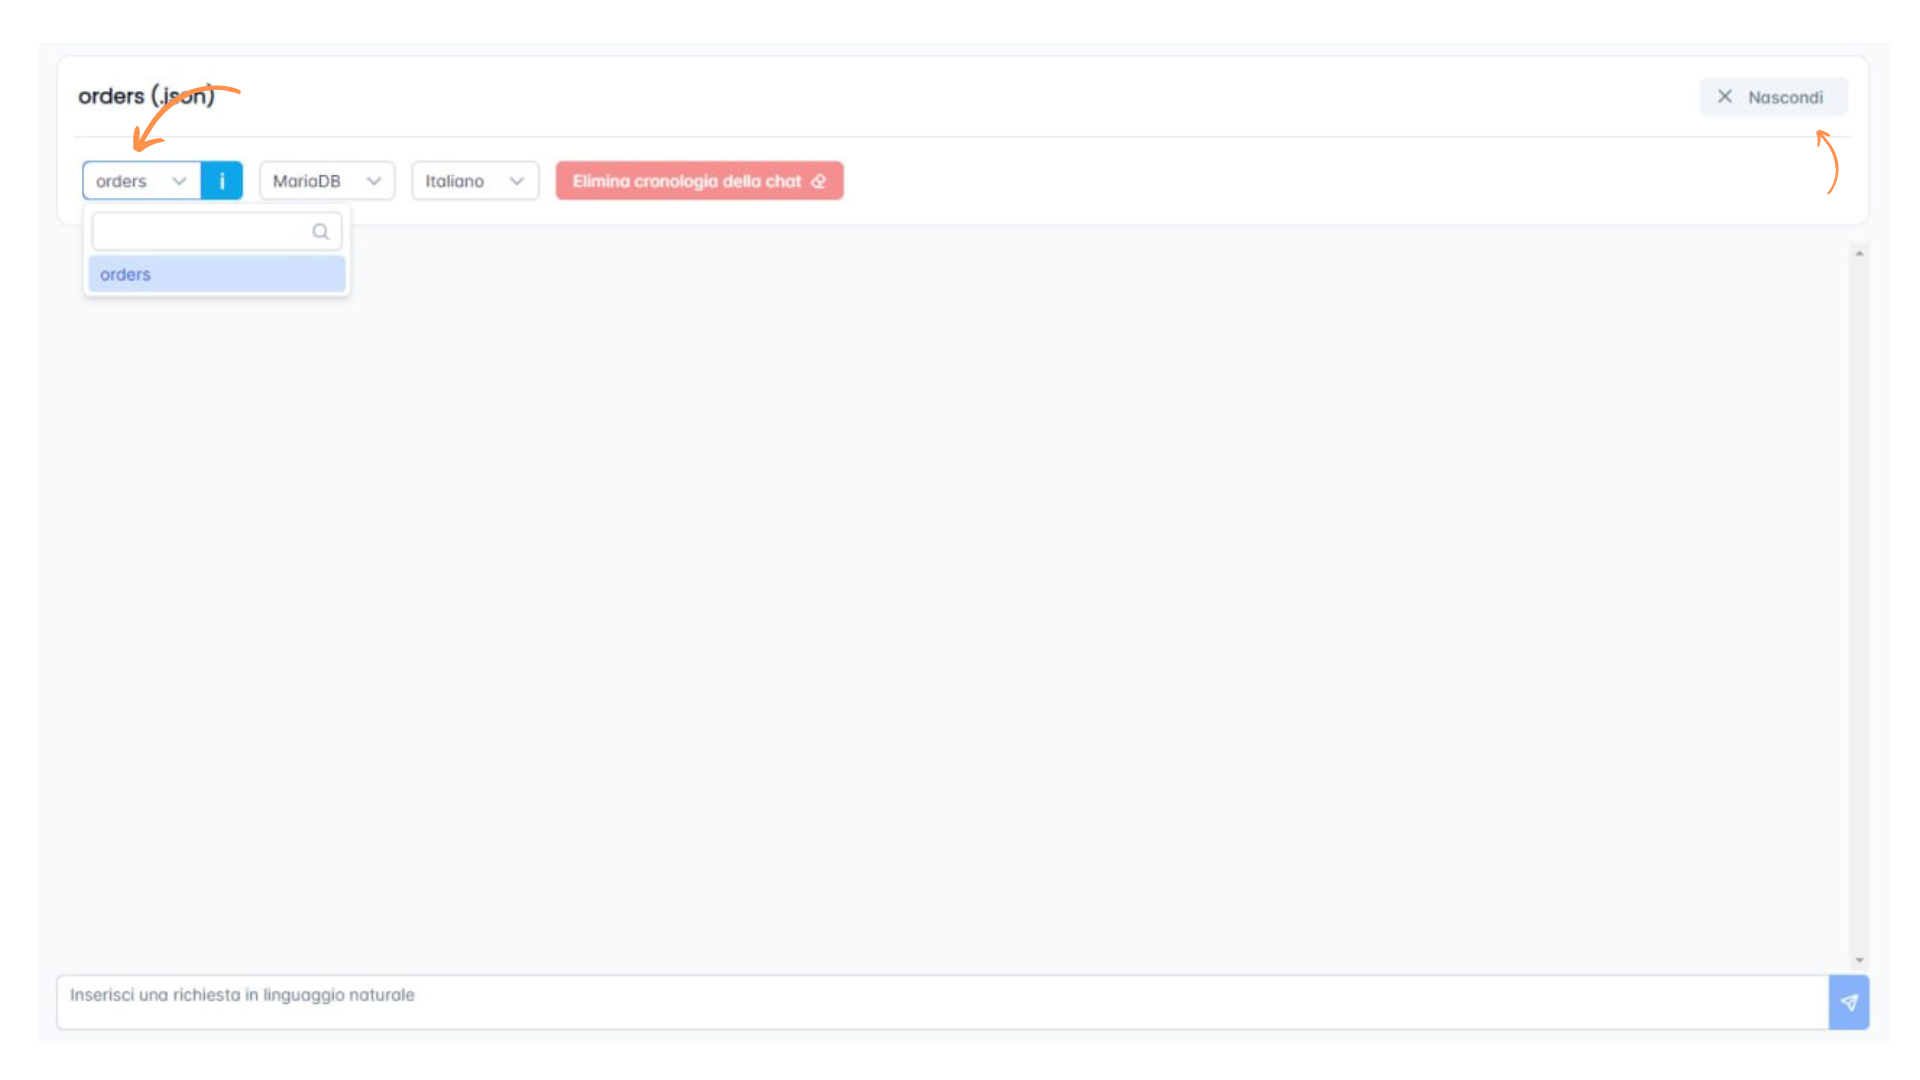
\includegraphics[width=1\textwidth]{assets/cambio_dizionariodati.png}
  \caption{Menu di cambio dizionari dati}
\end{figure}

\subsubsection{Accesso ad informazioni aggiuntive sul dizionario dati scelto}

È possibile accedere a delle informazioni aggiuntive di quello specifico dizionario cliccando il bottone "Mostra" in alto a destra nella chat e una volta aperto il menù il dizionario dati sarà la prima voce a sinistra delle quattro presenti e selezionando la "i" con sfondo azzurro a destra della freccia appariranno le informazioni ricercate. Questa operazione amplierà le informazioni nella scheda mostrando: il nome, una descrizione in linguaggio naturale delle informazioni contenute nel dizionario dati e una lista delle tabelle con le relative descrizioni delle informazioni al loro interno. Il nome delle tabelle è a sinistra in grassetto mentre la descrizione è quella che segue i due punti. Per chiudere le informazioni del dizionario dati e tornare alla chat si può: 1) cliccare la "x" affianco al box del dizionario dati dove prima si trovava la "i" per accedere ai dettagli del dizionario. Questa azione è consigliabile se è ancora necessaria l'interazione con il menù per cambiare dizionario dati, lingua o DBMS. 2).

\begin{figure}[H]
  \centering
  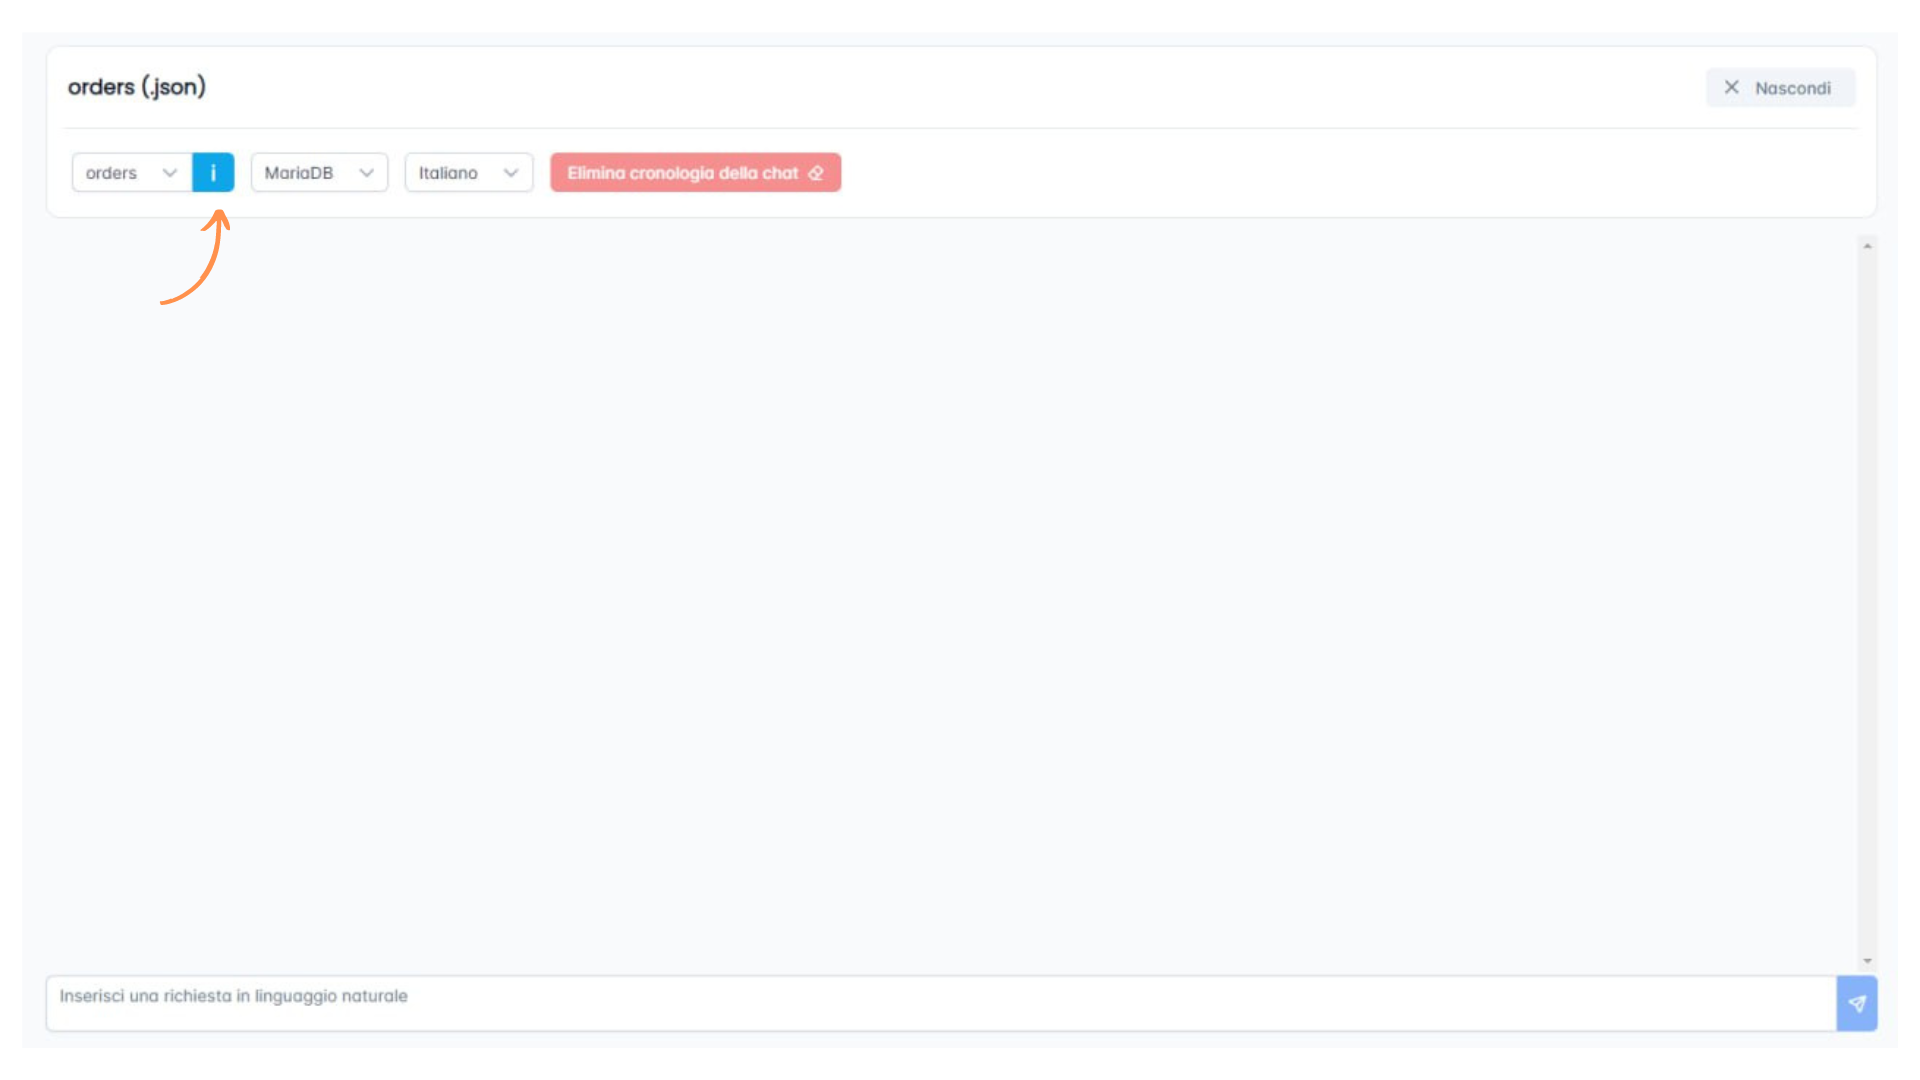
\includegraphics[width=1\textwidth]{assets/info_dizionario.png}
  \caption{Menu di informazioni aggiuntive sul dizionario dati}
\end{figure}

\subsubsection{Selezione/cambio DBMS}

È possibile selezionare il DBMS cliccando il bottone "Mostra" in alto a destra della chat che aprirà un menù con 4 voci di cui la seconda riguarda i DBMS. Quello che si legge al momento dell'apertura del menù è quello che il sistema ha usato fino a quel momento per generare i prompt. Se si vuole cambiare, si deve cliccare la freccia verso il basso a destra del nome attuale del DBMS. Questa operazione aprirà un menù a tendina con i diversi DBMS supportati dal sistema tra i quali si può scegliere. Per selezionare uno, basta cliccare con il tasto destro sopra al nome. I DBMS che sono supportati dal sistema e che possono essere selezionati sono: PostgreSQL, MariaDB, Microsoft SQL Server, Oracle DB e SQLite. Una volta selezionato il DBMS desiderato, se non si vuole scegliere anche una lingua o un dizionario dati, per tornare alla chat è possibile cliccare il tasto in alto a destra "Nascondi" che chiuderà il menù.

\begin{figure}[H]
  \centering
  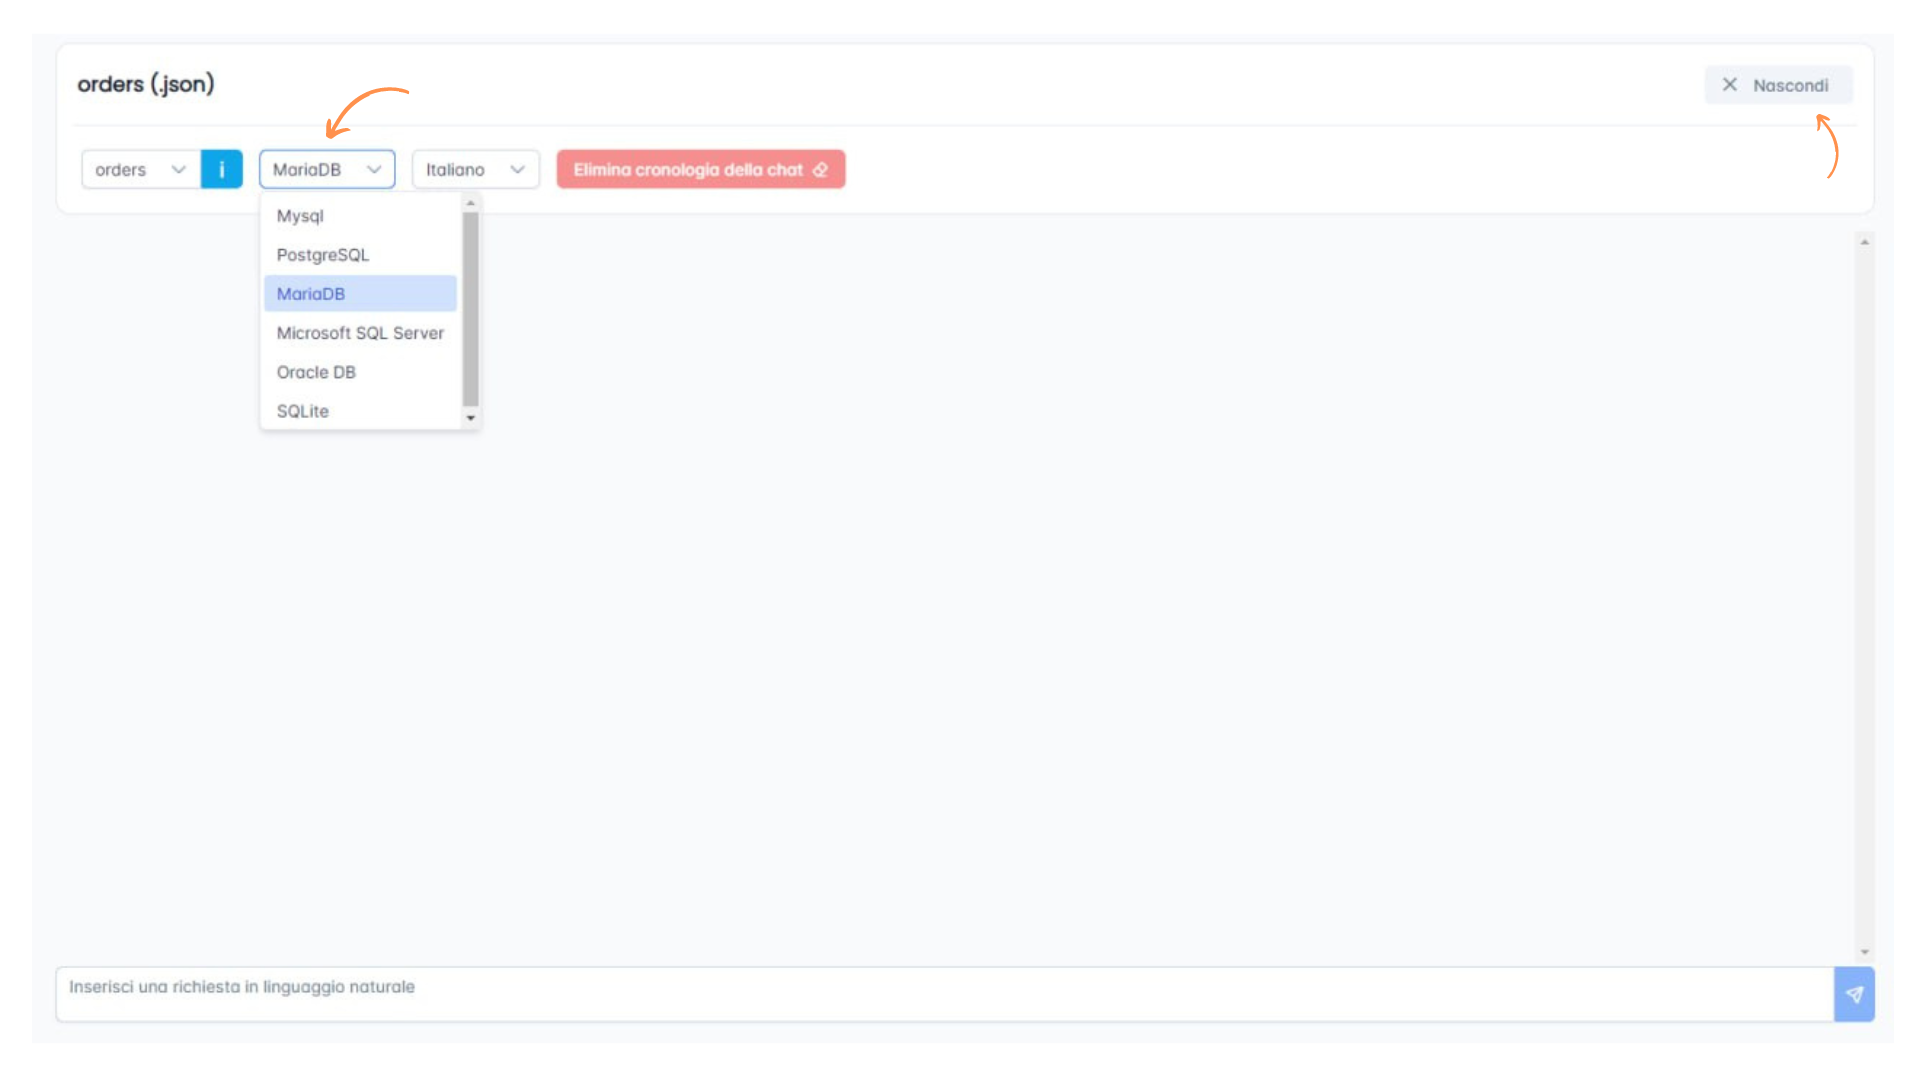
\includegraphics[width=1\textwidth]{assets/cambio_dbms.png}
  \caption{Menu di cambio DBMS}
\end{figure}

\subsubsection{Selezione/cambio lingua}

È possibile selezionare una lingua cliccando il bottone "Mostra" in alto a destra della chat che aprirà un menù con 4 voci di cui la terza riguarda la lingua. Quella che si legge al momento dell'apertura del menù è quella che il sistema ha usato fino a quel momento per generare i prompt. Se si vuole cambiare, si deve cliccare la freccia verso il basso a destra della lingua attuale. Questa operazione aprirà un menù a tendina con le diverse lingue supportate dal sistema tra le quali si può scegliere. Per selezionare una lingua, basta cliccare con il tasto destro sopra al nome. Le lingue che sono supportate dal sistema e che possono essere selezionate sono: Inglese, Italiano, Francese, Spagnolo e Tedesco. Una volta selezionata la lingua desiderata, se non si vuole scegliere anche un DBMS o un dizionario dati, per tornare alla chat è possibile cliccare il tasto in alto a destra "Nascondi" che chiuderà il menù.

\begin{figure}[H]
  \centering
  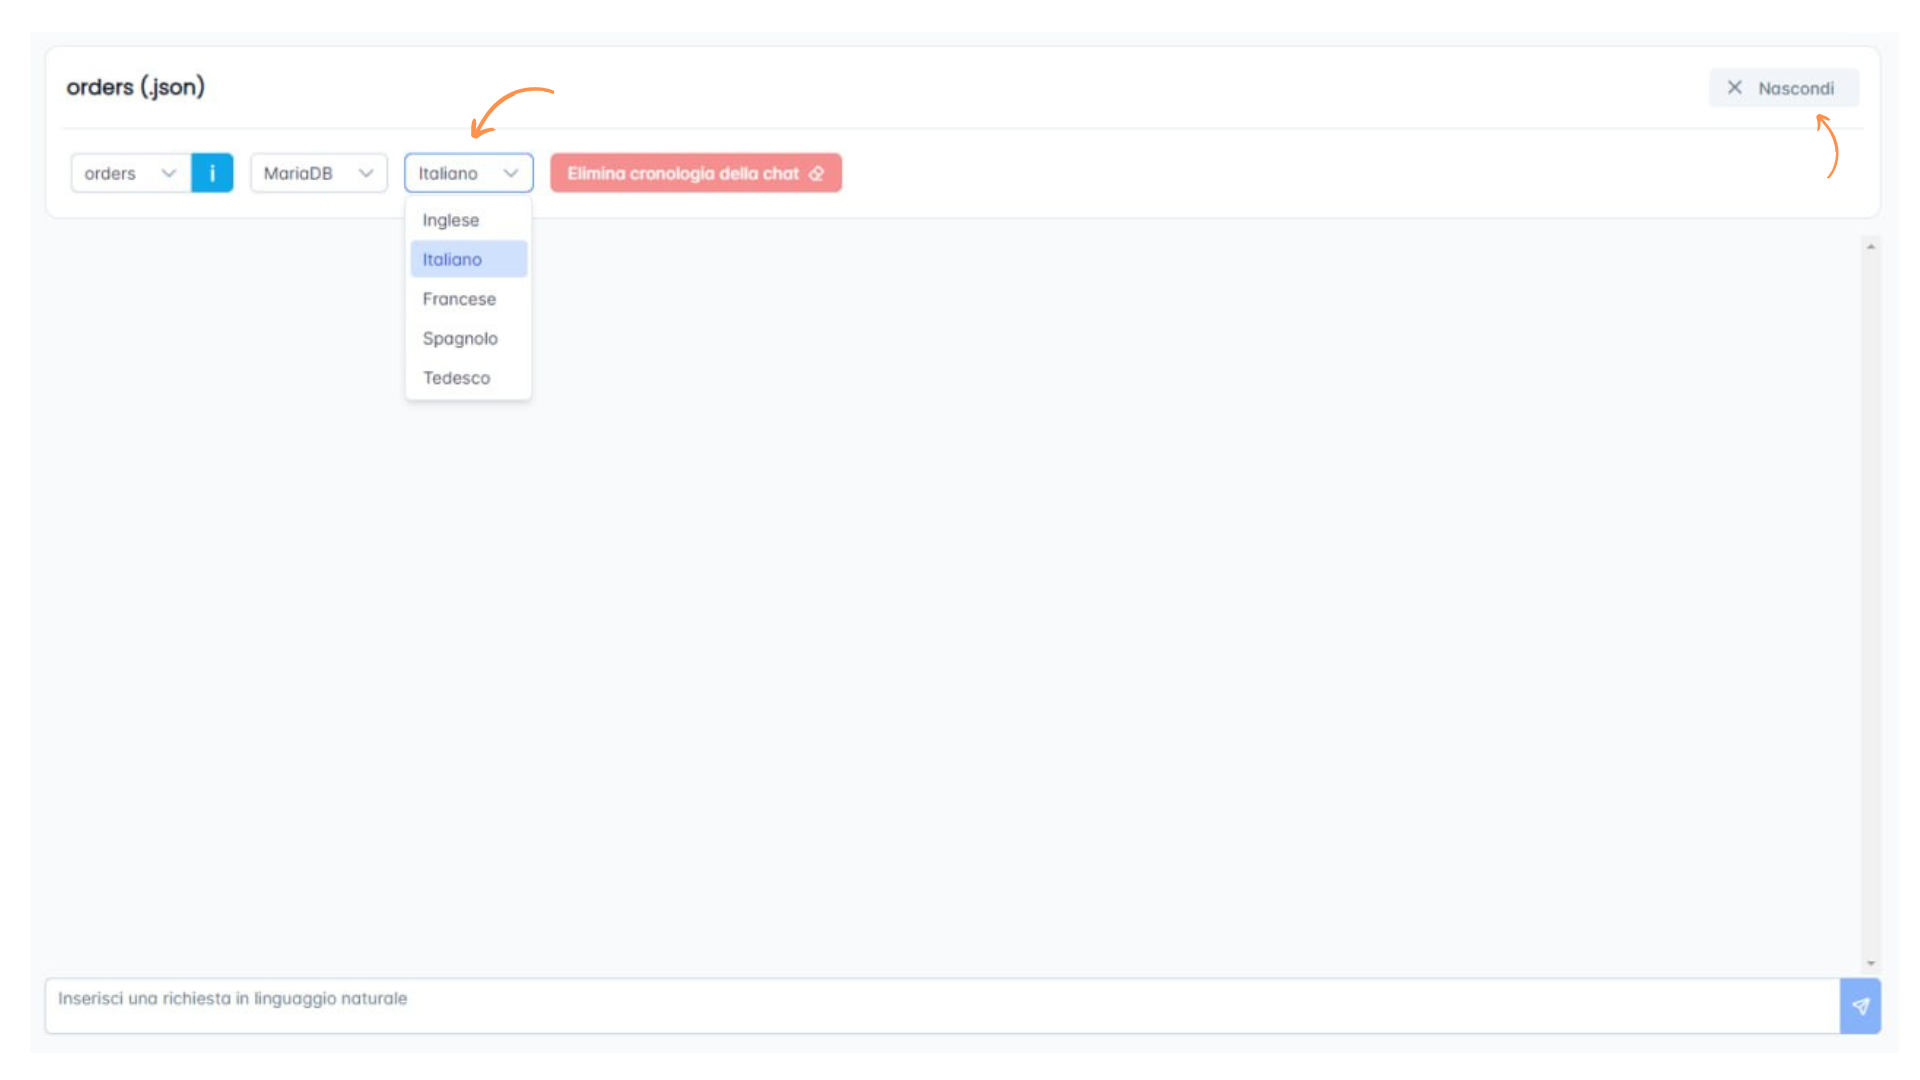
\includegraphics[width=1\textwidth]{assets/cambio_lingua.png}
  \caption{Menu di cambio lingua}
\end{figure}

\subsection{Funzionalità disponibili dopo l'interazione con la chat}

\begin{enumerate}
  \item Eliminazione della chat
  \item Copia del prompt
\end{enumerate}

\subsubsection{Eliminazione della chat}

Dopo l'interazione con il sistema, l'utente può voler eliminare le richieste e i prompt generati fino a quel momento ripulendo quindi la chat. Questo si può fare cliccando il bottone "Mostra" in alto a destra nella chat e una volta aperto il menù cliccando il bottone rosso nominato: "Elimina cronologia della chat". Questa scelta cancellerà il contenuto di tutte le richieste e le risposte fino a quel momento che andranno perse completamente dal sistema.

\begin{figure}[H]
  \centering
  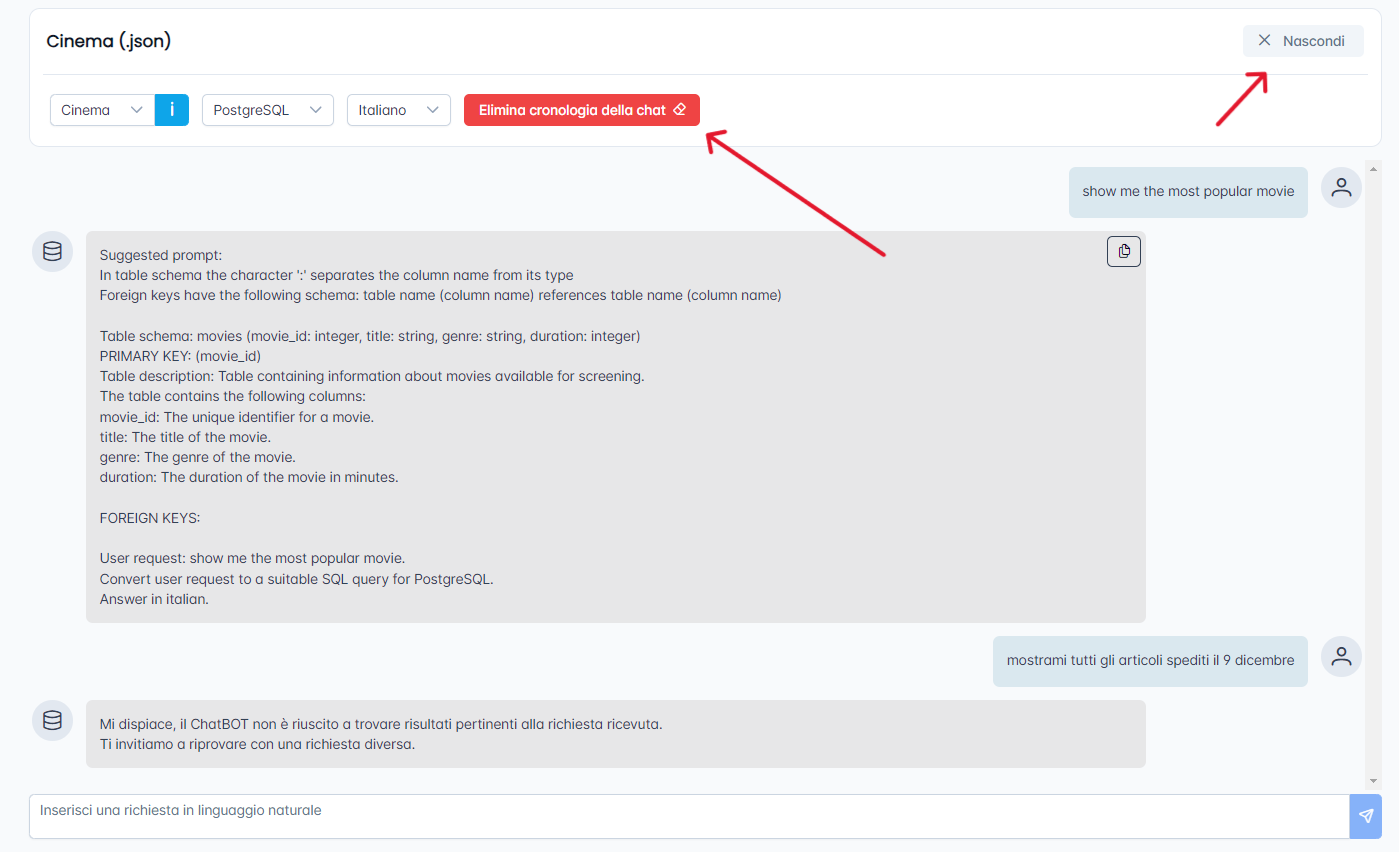
\includegraphics[width=1\textwidth]{assets/elimina_chat.png}
  \caption{Eliminazione della cronologia della chat}
\end{figure}

\subsubsection{Copia del prompt}

Dopo che è stato generato un prompt, è possibile copiare la risposta restituita cliccando sull'icona bianca in alto a destra in modo da poter copiare in locale il testo così formattato e incollarlo successivamente in altri applicativi e/o in un sistema di intelligenza artificiale come ChatGpt o altri Large Language Model.

\begin{figure}[H]
    \centering
    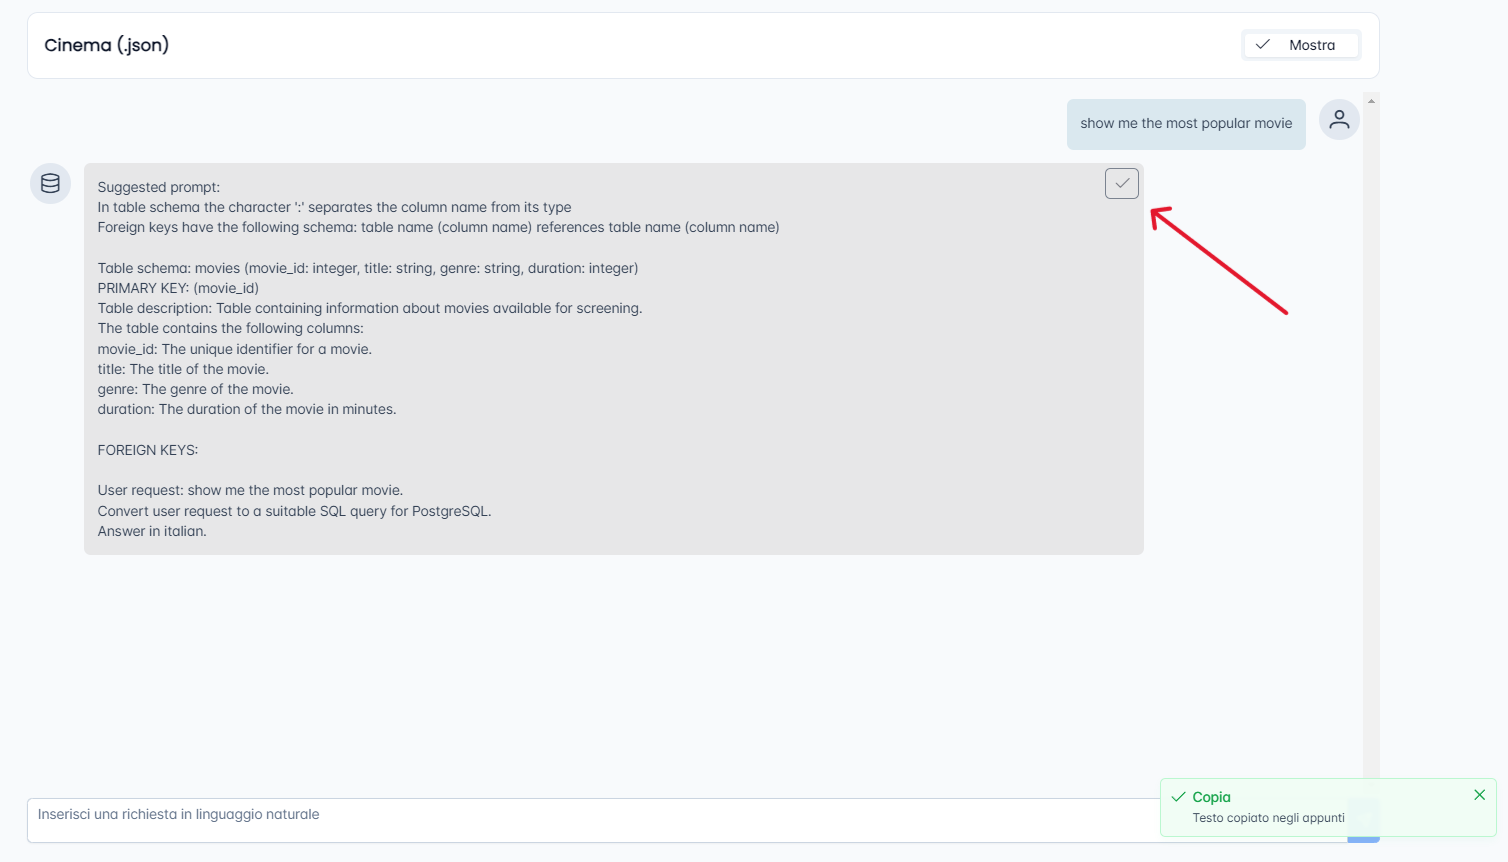
\includegraphics[width=1\textwidth]{assets/copia.png}
    \caption{copia del prompt}
  \end{figure}